%%%%%%%%%%%%%
%  Frame 1  %
%%%%%%%%%%%%%
\begin{frame}
\frametitle{Caos in Dimensione 3}
\framesubtitle{Teorema di Shil'nikov}
A. Arneodo et al. dimostrano che rilassando la \ref{en:c2}) si può ottenere un attrattore strano con $n=3$.\\
Rilassare la 2) significa poter scegliere $a_{ij} < 0$.
\begin{block}{Teorema di Shil'nikov}
Se il sistema linearizzato in $\v{x}^*_s$ è della forma (Saddle-Focus):
\[
    \begin{cases}
	\dot{x} = \left(\rho  + i\omega\right) x \\
	\dot{y} = \left(\rho  - i\omega\right) y \\
	\dot{z} = \lambda z
    \end{cases} 
    \qquad \lambda > -\rho > 0
\] 
ed $\exists$ curva $\Gamma_0$ che lascia $\v{x}^*_s$ e vi ritorna per $t\to \infty$ allora ogni intorno di $\Gamma_0$ contiene un insieme numerabile di orbite periodiche instabili (di tipo sella).
\end{block}
\end{frame}

%%%%%%%%%%%%%
%  Frame 2  %
%%%%%%%%%%%%%
\begin{frame}
\frametitle{Caos in Dimensione 3}
\framesubtitle{Metodo Euristico di costruzione dell'attrattore}
\[
    r_i = 1 \qquad \frac{\text{d} x_i}{\text{d} t} = x_i \sum_{j=1}^{3} a_{ij}(1-x_j) 
.\] 
\begin{itemize}
    \item Si fissano casualmente 8 di 9 parametri di $a_{ij}$:
	\[
	    a_{ij} =\begin{pmatrix}
	        0.5 & 0.5 & 0.1 \\
	        -0.5 & -0.1 & 0.1 \\
	        \mu & 0.1 & 0.1 \\
	    \end{pmatrix}
	\] 
    \item $\mu$ si fissa in modo da avere
	\begin{itemize}
	    \item $\mu  > \mu_0$ $\implies$ Uno dei punti $Q_{ij}\equiv A$ di tipo "Saddle-Focus".
	    \item $\mu > \mu_H > \mu_0$ $\implies$ Il punto $B$: $x_i=1$ $\forall i = 1, 2, 3$ con biforcazione di Hopf.
	\end{itemize}
    \item Si fa variare $\mu$ al di sopra della biforcazione.
\end{itemize}
\end{frame}

%%%%%%%%%%%%%
%  Frame 3  %
%%%%%%%%%%%%%
\begin{frame}
\frametitle{Caos in Dimensione 3}
\framesubtitle{Formazione dell'orbita omoclinica}
\begin{figure}[H]
    \centering
    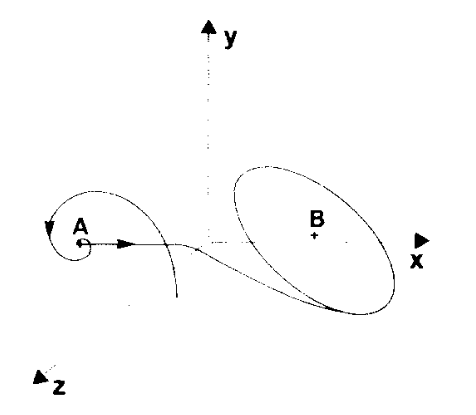
\includegraphics[width=0.4\textwidth]{figures/omo1.png}
    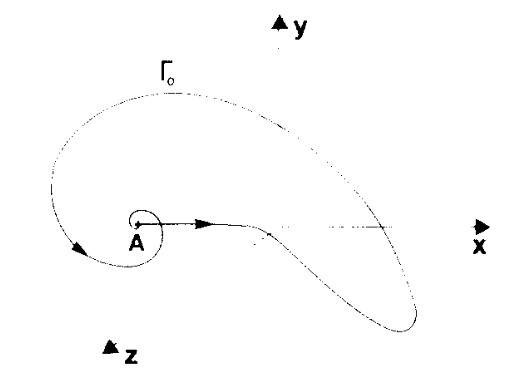
\includegraphics[width=0.4\textwidth]{figures/omo2.png}
    \caption{Costruzione grafica della curva $\Gamma_0$ del teorema di Shil'nikov (Arneodo et al). }
    \label{fig:figures-omo2-png}
\end{figure}
\begin{center}
Simulazione del sistema al variare di $\mu$ \textcolor{blue}{\href{run:link/Animated_trans.html}{(trans)}}, \textcolor{blue}{\href{run:link/Animated_no_trans.html}{(no trans)}}
\end{center}
\end{frame}

%%%%%%%%%%%%%
%  Frame 4  %
%%%%%%%%%%%%%
\begin{frame}
\frametitle{Caos in Dimensione 3}
\framesubtitle{Costruzione dell'attratore}
\begin{figure}[H]
    \centering
    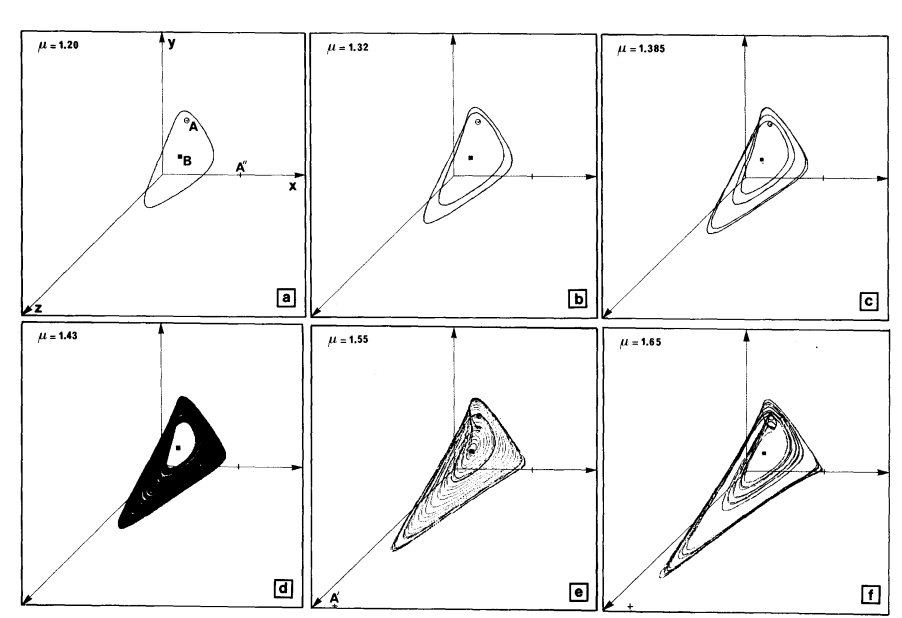
\includegraphics[width=0.8\textwidth]{figures/Hopf.png}
    \caption{Formazione dell'attrattore strano a partire dal sistema della slide precedente (Arneodo et al.)}
    \label{fig:figures-Hopf-png}
\end{figure}
\end{frame}

%%%%%%%%%%%%%
%  Frame 4  %
%%%%%%%%%%%%%
\begin{frame}
\frametitle{Caos in dimensione 4}
\framesubtitle{Estensione dei parametri ottenuti in dimensione 3}
\begin{block}{Coste et al.:}
Ogni sistema di LV di dimensione $n+1$ con $r_i = r_j$ $i, j = 1, \ldots, n+1$ può essere ridotto ad un sistema di LV di dimensione $n$ e viceversa.
\end{block}
\vspace{1em}
$\implies$ è possibile ottenere caos in dimensione 4 rispettando anche le richieste \ref{en:c1}), \ref{en:c2}), \ref{en:c3}).
\end{frame}

%%%%%%%%%%%%%
%  Frame 5  %
%%%%%%%%%%%%%
\begin{frame}
\frametitle{Caos in dimensione 4}
\framesubtitle{Generalizzare i risultati di Arneodo et al.}
\begin{block}{Alcuni risultati di Vano et al.}
\begin{itemize}
    \item Generalizzare il modello:
	\begin{itemize}
	    \item $r_i \neq r_j$.
	\end{itemize}
    \item Analisi numerica:
	\begin{itemize}
	    \item Massimizzare l'esponente di Lyapunov positivo.
	    \item Vincolare le popolazioni $x_i \ge x_{\text{lim}}$ (evitare estinzione).
            \item Analisi della rarità delle soluzioni caotiche nello spazio dei parametri.
	\end{itemize}
\end{itemize}
\end{block}
\end{frame}

%%%%%%%%%%%%%
%  Frame 6  %
%%%%%%%%%%%%%
\begin{frame}
\frametitle{Caos in dimensione 4}
\framesubtitle{Analisi numerica}
\begin{itemize}
    \item $r_i$, $a_{ij}$: 20 parametri iniziali.
	\begin{itemize}
	    \item $r_0=1$ 
	    \item $a_{ii} = 1$ 
	\end{itemize}
	Restano 15 parametri liberi.
    \item Ricerca numerica nello spazio dei parametri:
	\begin{itemize}
	    \item Aggiornare i parametri.
	    \item Simulare il sistema.
	    \item Fermare la simulazione se $x_i < x_{\text{lim}}$ (e tornare in cima).
	    \item Calcolare gli esponenti di Lyapunov.
	    \item Salvare la configurazione $\overline{r}_i, \overline{a}_{ij}$ che massimizza gli esponenti.
	\end{itemize}
\end{itemize}
\end{frame}

%%%%%%%%%%%%%
%  Frame 7  %
%%%%%%%%%%%%%
\begin{frame}
\frametitle{Caos in dimensione 4}
\framesubtitle{Risultati ottenuti}
\[
    r =\begin{bmatrix}
        1 \\
        0.72 \\
        1.53 \\
        1.27 \\
    \end{bmatrix} \qquad 
    a =\begin{bmatrix}
        1 & 1.09 & 1.52 & 0 \\
        0 & 1 & 0.44 & 1.36 \\
        2.33 & 0 & 1 & 0.47 \\
        1.21 & 0.51 & 0.35 & 1 \\
    \end{bmatrix}
\] 
\vspace{1em}
\[
    LEs = \left[0.0203, 0, -0.2748, -1.0289\right]; \qquad  \sum_{}^{} LEs = -1.2834
.\] 
\vspace{0.5em}
\[
    D_{KY} = 2.074
.\] 
\vspace{0.5em}
\begin{center}
\textcolor{blue}{\href{run:link/LV_simu.html}{Simulazione del sistema\ldots}}
\end{center}
\begin{center}
\textcolor{blue}{\href{run:link/Max_LE.html}{Distribuzione degli esponenti di Lyapunov}}
\end{center}
\end{frame}

%%%%%%%%%%%%%
%  Frame 8  %
%%%%%%%%%%%%%
\begin{frame}
\frametitle{Ottenere il Grafico di Biforcazione}
Per ottenere il grafico di biforcazione si utilizza un parametro $s$:
\[
    a_{ij} = \begin{cases}
	a_{ij} &\text{ se } i = j\\
	s\cdot a_{ij} & \text{ se } i \neq j
    \end{cases}
.\] 
$\forall s \in S \subset \mathbb{R}$ (intervallo arbitrario):
\begin{itemize}
    \item Si simula il sistema.
    \item Si scartano le prime $n$ iterazioni (termalizzazione).
    \item Si salvano tutti i massimi locali di una delle variabili al variare di $s$. 
\end{itemize}
\end{frame}

%%%%%%%%%%%%%
%  Frame 9  %
%%%%%%%%%%%%%
\begin{frame}
\frametitle{Rarità del Caos e Grafico di Biforcazione}
\begin{figure}[H]
    \centering
    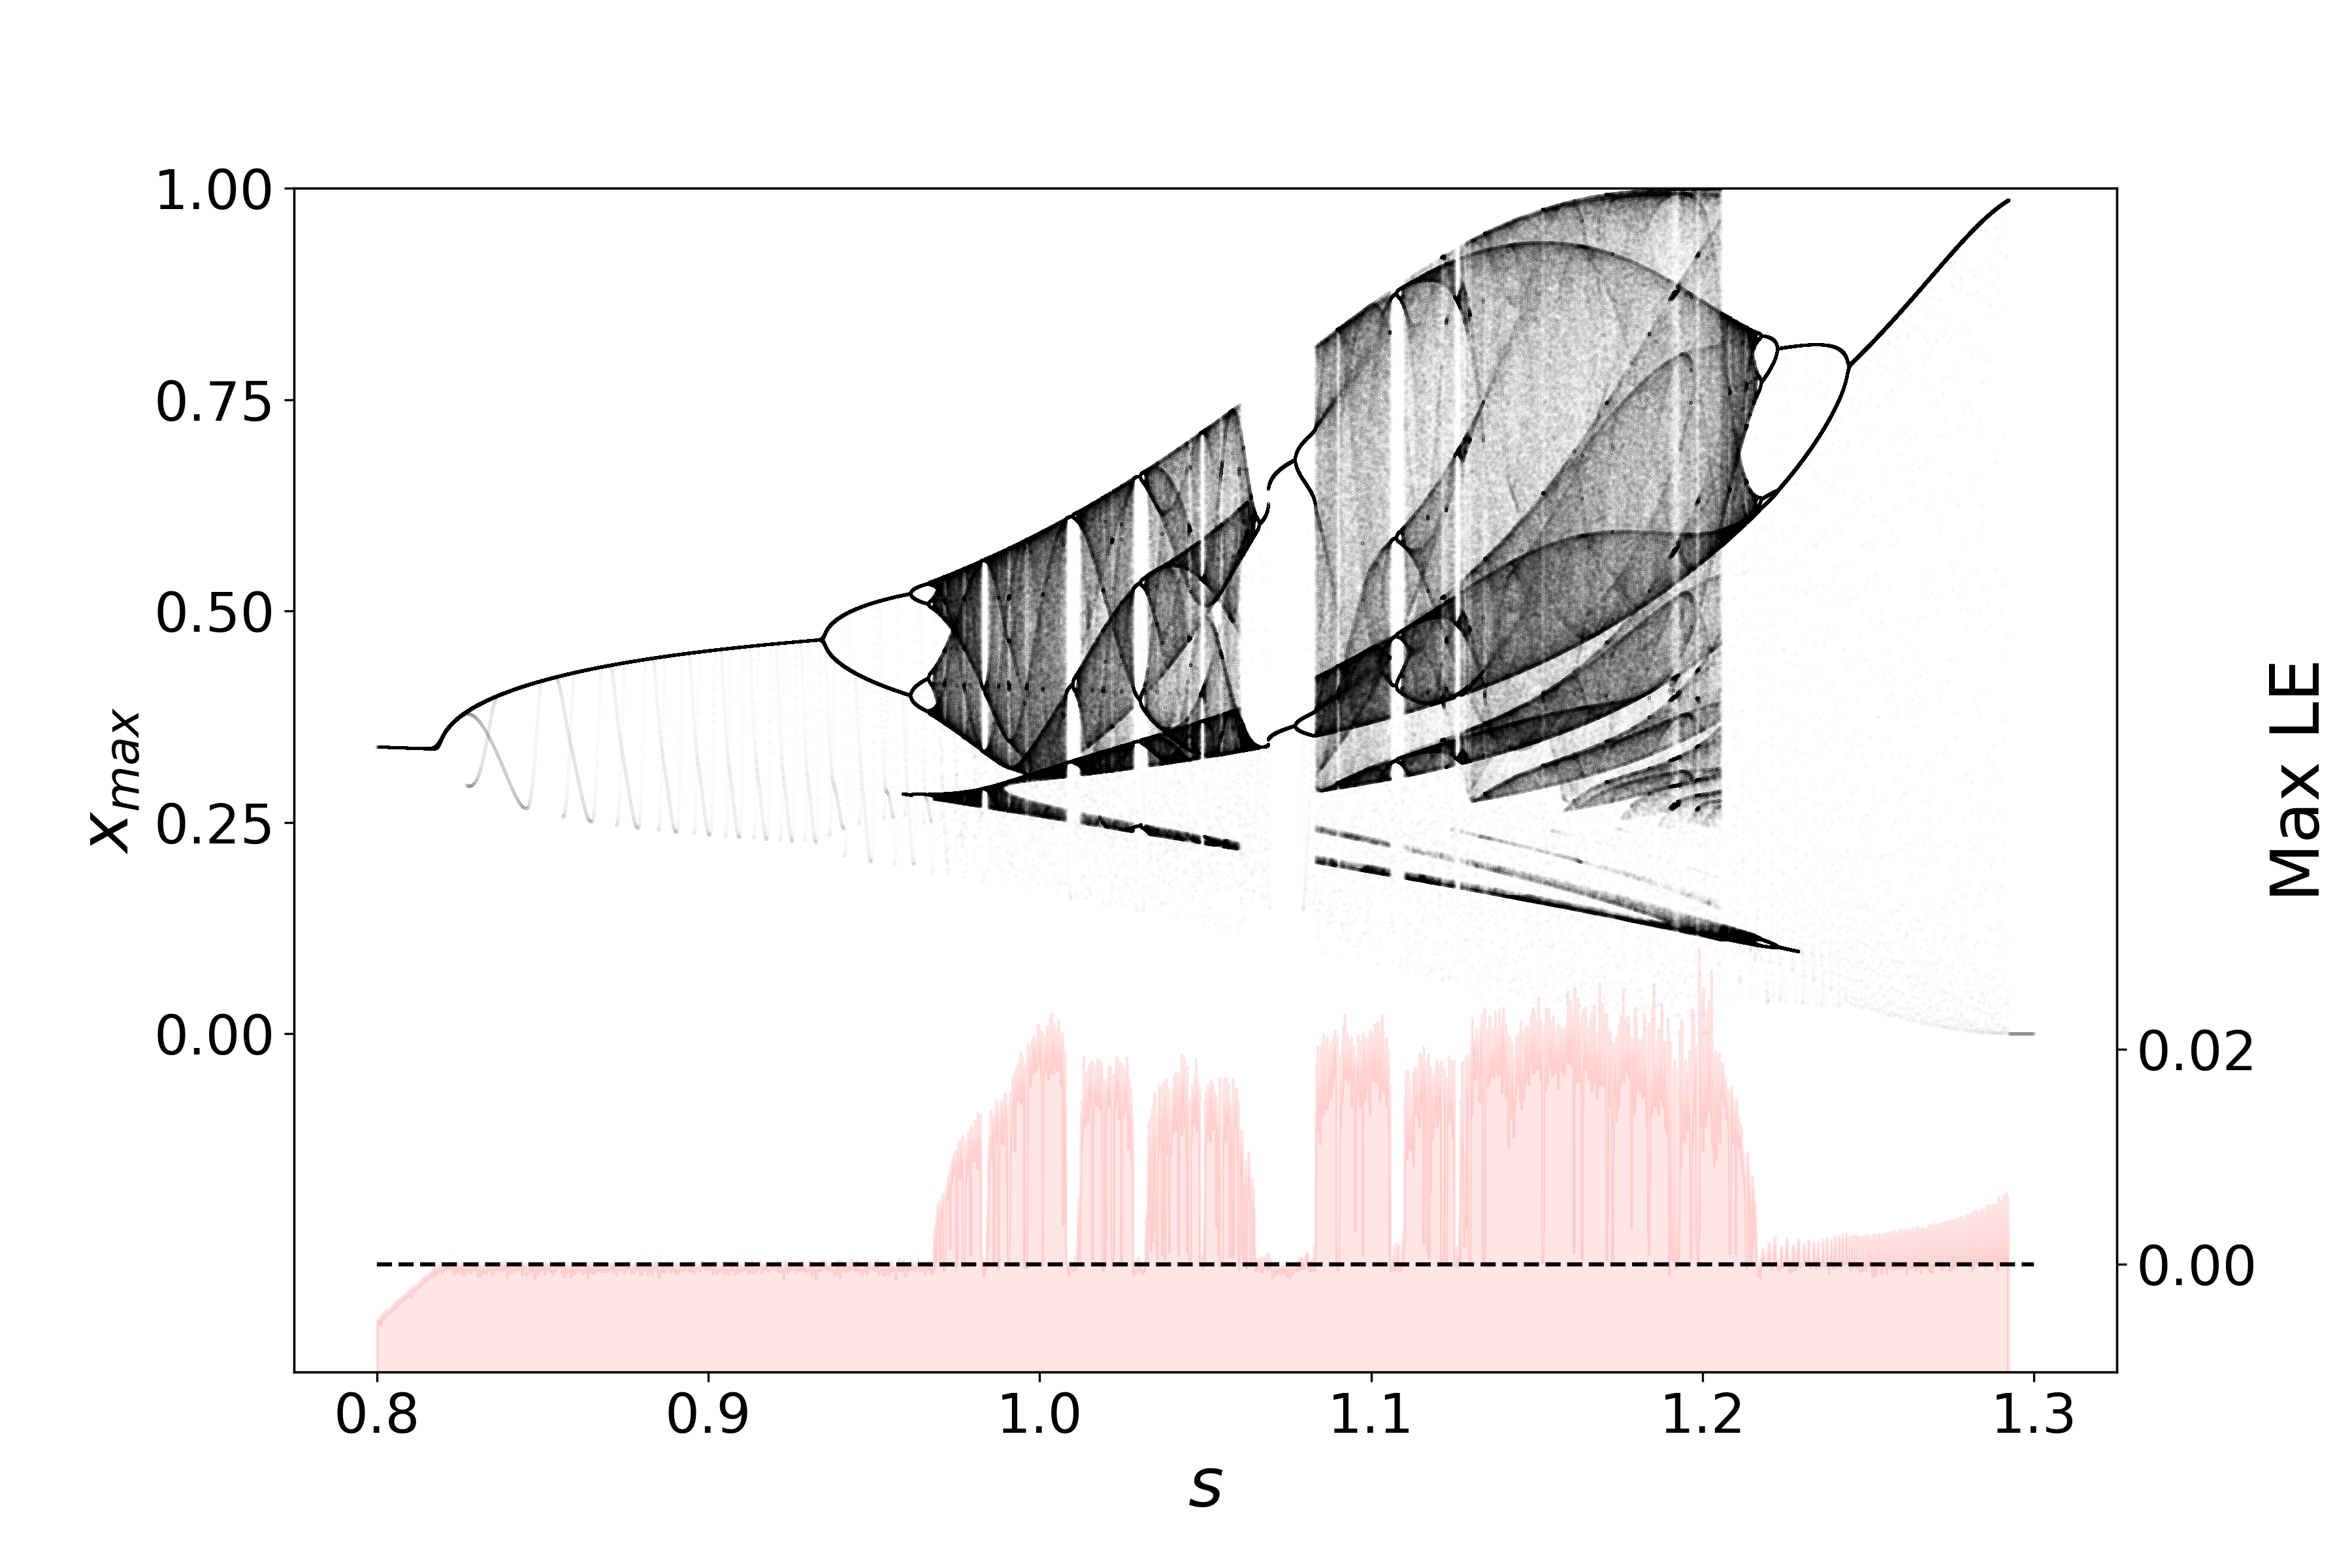
\includegraphics[width=\textwidth]{figures/bif_diag.png}
\end{figure}
\end{frame}
